\documentclass[10pt,letterpaper]{article}
\usepackage[margin=0.75in]{geometry}
\usepackage{amsmath,amssymb,graphicx,booktabs,xcolor,fancyhdr,hyperref}
\definecolor{navy}{HTML}{17364B}
\hypersetup{colorlinks=true,linkcolor=navy,urlcolor=navy}
\pagestyle{fancy}\fancyhf{}\lhead{\small THREE-DIMENSIONAL LINEAR DISPERSION}\rhead{\small Numerical study}\cfoot{\thepage}
\setlength{\headheight}{14pt}\setlength{\parindent}{0pt}\setlength{\parskip}{6pt}
\newcommand{\norm}[1]{\left\|#1\right\|}
\newcommand{\MassError}{$1.11\times10^{-16}$}
\newcommand{\SymmetryError}{$1.76\times10^{-16}$}
\newcommand{\PlaneError}{$2.18\times10^{-15}$}
\newcommand{\ReverseError}{$6.69\times10^{-16}$}
\newcommand{\QuadError}{$3.91\times10^{-9}$}
\newcommand{\PeakPercent}{0.556}
\newcommand{\Runtime}{12.4}
\newcommand{\FinalRows}{$1$ & unshifted & 0.473 & 3.598 & 3.598 & 3.866 \\
$1$ & x shift & 0.438 & 3.891 & 3.598 & 4.140 \\
$1$ & z shift & 0.414 & 4.849 & 4.849 & 3.090 \\
$-1/3$ & unshifted & 0.481 & 3.598 & 3.598 & 3.629 \\
$-1/3$ & x shift & 0.444 & 3.891 & 3.598 & 3.919 \\
$-1/3$ & z shift & 0.303 & 4.849 & 4.849 & 4.872 \\
$0$ & unshifted & 0.467 & 3.598 & 3.598 & 3.598 \\
$0$ & x shift & 0.433 & 3.891 & 3.598 & 3.891 \\
$0$ & z shift & 0.346 & 4.849 & 4.849 & 3.598 \\}
\newcommand{\GridRows}{$32^3$ & $1.89\times10^{-1}$ & $2.05\times10^{-1}$ & $1.68\times10^{-1}$ \\
$64^3$ & $7.75\times10^{-6}$ & $8.24\times10^{-6}$ & $7.38\times10^{-6}$ \\
$96^3$ & $2.13\times10^{-14}$ & $2.15\times10^{-14}$ & $1.90\times10^{-14}$ \\}
\newcommand{\DomainRows}{$1$ & $5.87\times10^{-3}$ & $2.00\times10^{-5}$ & $2.07\times10^{-4}$ \\
$-1/3$ & $3.70\times10^{-2}$ & $1.71\times10^{-5}$ & $1.55\times10^{-5}$ \\
$0$ & $3.95\times10^{-3}$ & $1.49\times10^{-7}$ & $5.58\times10^{-7}$ \\}

\begin{document}
{\color{navy}\Huge Numerical solutions in three variables}\par
{\Large The linear optical model in the Dysthe research context}\par
{\small Computed September 9, 2026 \quad | \quad Reproducible Torch experiments}
\vspace{8pt}

\textbf{Scope.} This report computes the linearization of equation (1.27) in
Mosincat--Pilod--Saut, \emph{On Third Order Nonlinear Schr\"odinger Equations},
using the supplied file \texttt{Dysthe3D-2.pdf}. It contains nine Gaussian runs
and one two-packet example. These are numerical solutions of a linear initial-value
problem; they are not simulations of the full nonlinear Dysthe water-wave system.
The optical model uses three independent coordinates $(x,y,z)$ and evolution variable
$t$, after the physical propagation/time coordinates have been renamed in the paper.

\section*{Reading the plots: what is the envelope?}
The complex field $E$ describes the slowly varying amplitude and phase of an optical
wave. Its magnitude $|E|$ is the \textbf{envelope amplitude}, not a velocity.
Imagine rapid oscillations whose heights gradually grow and shrink: the envelope
follows those heights rather than tracing every oscillation.

\begin{center}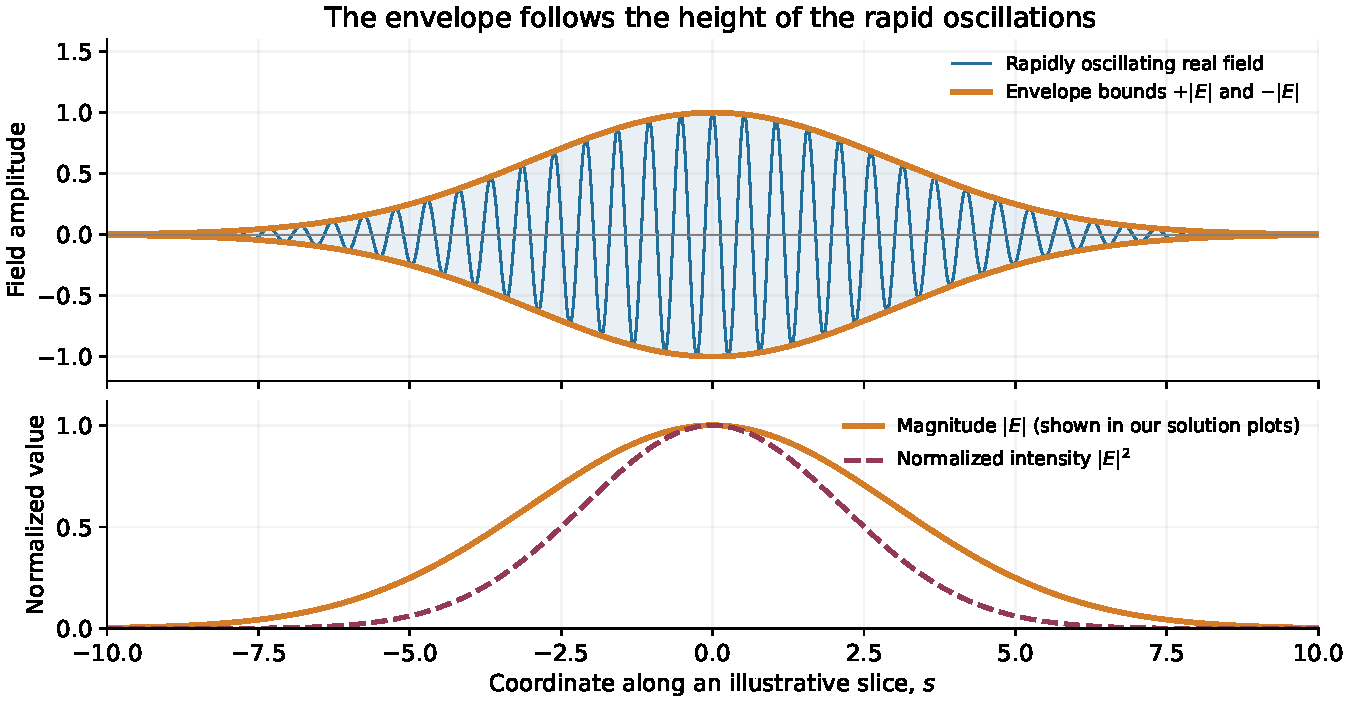
\includegraphics[width=\linewidth]{figures/envelope_explanation.pdf}\end{center}
\textbf{Figure 1.} An illustrative one-coordinate slice at a fixed instant.
The blue oscillations lie between the orange curves $+|E|$ and $-|E|$.
The lower panel separates envelope magnitude from intensity. This diagram uses
$E(s)=e^{-s^2/18}$ and an illustrative carrier $\cos(12s)$; the carrier frequency
is chosen for visibility and is not a physical parameter inferred from the simulation.

A real optical field is reconstructed schematically as
$\operatorname{Re}\{E e^{i\phi_{\mathrm{carrier}}}\}$: the envelope supplies its amplitude
and an additional phase. Our solver evolves $E$; the subsequent magnitude plots
show $|E|$ without drawing the rapid carrier oscillations. All reported amplitudes
are dimensionless, with the initial Gaussian peak normalized to one.

Optical intensity is proportional to $|E|^2$. A peak magnitude of $0.47$ therefore
corresponds to about $0.22$ of the initial peak intensity. A falling peak can reflect
spreading while total integrated intensity remains constant. How fast the packet
moves is a separate question, described by its group velocity.

\newpage
\section*{For water: a set of waves passing across the surface}
On water, a wave packet looks like several crests that become taller toward the
middle of a group and smaller toward its edges. The water surface is the oscillating
curve; the envelope is an imaginary outline of its local amplitude, not a second
surface. For a nearly sinusoidal wave, crest-to-trough height is approximately
\emph{twice} the envelope amplitude.

\begin{center}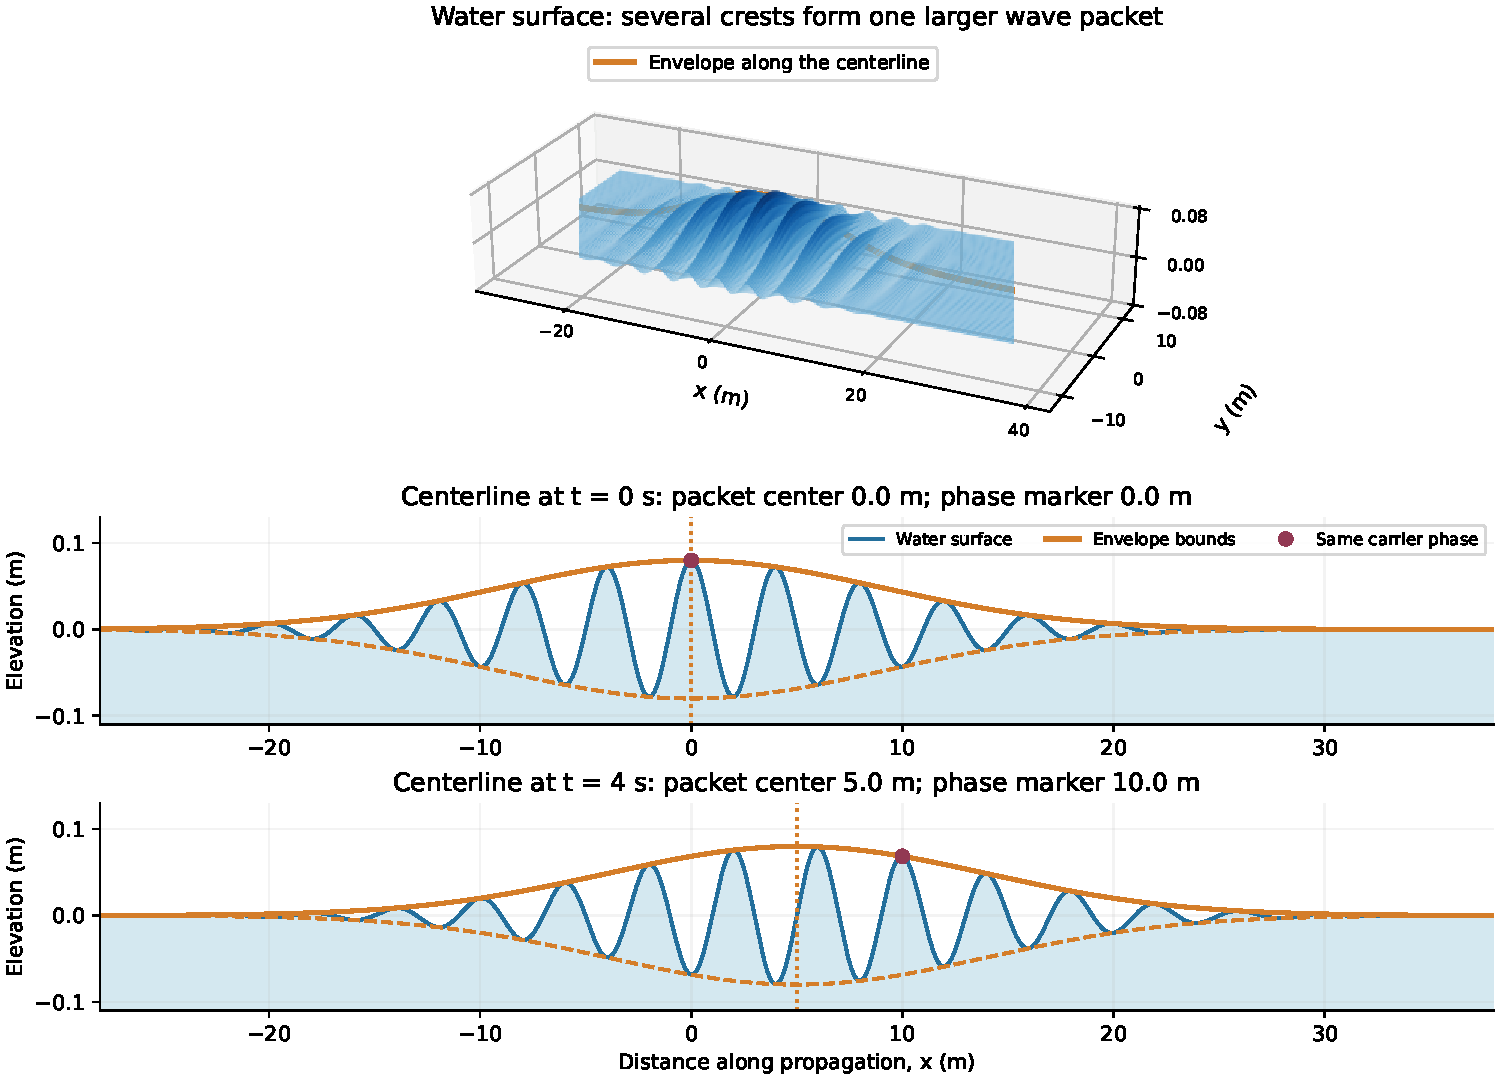
\includegraphics[width=.96\linewidth]{figures/water_packet.pdf}\end{center}
\textbf{Figure 2.} Illustrative deep-water gravity-wave packet. The perspective view
shows a surface over two horizontal coordinates; its vertical axis is elevation,
with vertical scale exaggerated. Below, the orange dotted line follows the packet
center and the red dot follows one carrier phase. The carrier phase advances faster
than the envelope. Neither marker follows a parcel of water.

For small-amplitude, narrowband gravity waves in deep water without currents,
$\omega_0=\sqrt{gk_0}$, $c_p=\omega_0/k_0$, and $c_g=c_p/2$. Individual crests
therefore pass through the group, growing and fading as they do so. This illustration
uses wavelength $4$ m, peak amplitude $0.08$ m and $g=9.81$ m/s$^2$:
$c_p\simeq2.50$ m/s and $c_g\simeq1.25$ m/s.

\textbf{Connection to this report.} The drawing uses the leading-order form
$\eta=A(x-c_gt,y)\cos(k_0x-\omega_0t)$ with a Gaussian $A$; it omits packet
spreading, nonlinear corrections and breaking. It is a fluid analogy, not an output
of our optical solver. Water-wave surface envelopes typically depend on two
horizontal coordinates and time; our numerical field uses three independent
coordinates. Source for the wave-group interpretation: R. Salmon,
\href{https://www-pord.ucsd.edu/rsalmon/111.textbook.pdf}{\emph{Introduction to Ocean Waves}},
Chapter 2, pp. 25--26.

\newpage
\section*{1. Equation and numerical model}
We solve
\begin{equation}
 iE_t+(1-i\varepsilon_1\partial_z)\Delta_\perp E-E_{zz}
       -i\varepsilon_2 E_{zzz}=0,
 \qquad \Delta_\perp=\partial_x^2+\partial_y^2.
 \label{eq:pde}
\end{equation}
With $\widehat E(\mathbf k)=\int E(\mathbf x)e^{-i\mathbf k\cdot\mathbf x}\,d\mathbf x$,
\begin{equation}
 \widehat E(\mathbf k,t)=e^{-it\omega(\mathbf k)}\widehat E_0(\mathbf k),\qquad
 \omega=(1+\varepsilon_1 k_z)(k_x^2+k_y^2)-k_z^2+\varepsilon_2k_z^3.
 \label{eq:prop}
\end{equation}
This matches the paper's symbol (6.6). Its equation (1.32) prints the opposite sign
on the mixed third derivative. We follow (1.27) and (6.6) consistently; this choice
must be retained when comparing with another implementation.

An FFT computes the initial coefficients once. For each requested $t$, we multiply
by the phase in \eqref{eq:prop} and perform an inverse FFT. Evolution of the retained
modes is exact up to floating-point arithmetic. There is no time-marching truncation
error; spatial sampling, finite-box effects, and sampling the peak remain relevant.
At a fixed total grid size $N$, $M$ snapshots cost $O(MN\log N)$.

\begin{center}
\begin{tabular}{ll}\toprule
Setting & Value \\\midrule
Computational box & $[-48,48)^3$, periodic \\
Production grid & $96^3$ points; $\Delta x=\Delta y=\Delta z=1$ \\
Arithmetic & Torch CPU, complex128, four threads \\
Evolution times & 25 snapshots, $t=0,0.25,\ldots,6$ \\
Parameters & $\varepsilon_1=1$; $\varepsilon_2\in\{1,-1/3,0\}$ \\
Initial Gaussian & $E_0=e^{-(x^2+y^2+z^2)/18}e^{i\mathbf q\cdot\mathbf x}$ \\
Frequency shifts & $\mathbf q=0$, $(\pi/6,0,0)$, $(0,0,\pi/6)$ \\\bottomrule
\end{tabular}
\end{center}
The shift is eight Fourier bins on the production box. All three initial magnitudes
are identical, with peak one. Positive $\varepsilon_2$ and $-\varepsilon_1/3$ connect
to the parameter cases in Theorem 5.1; the zero case is included as a linear comparison,
without extending that nonlinear theorem to it. All quantities are dimensionless.

\newpage
\section*{2. Peak evolution and parameter dependence}
The peak curves below are spatial grid maxima, not amplitudes at a fixed point.
All three parameter families spread over the observation window. The response to
a $z$-shift depends strongly on $\varepsilon_2$, even though the initial magnitudes
and norms are unchanged.
\begin{center}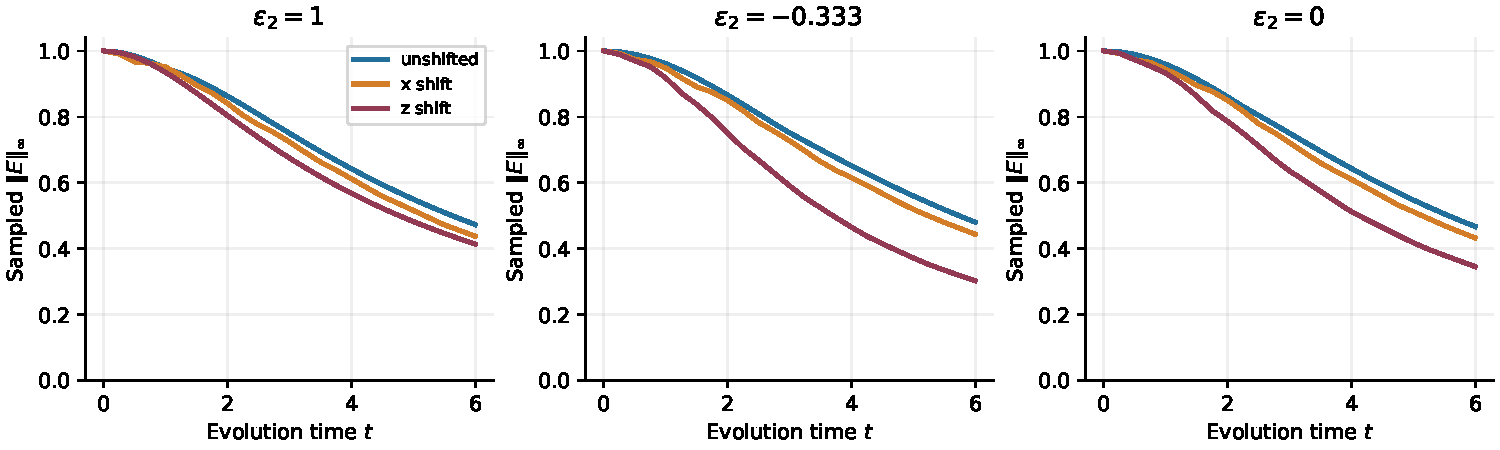
\includegraphics[width=\linewidth]{figures/peak_decay.pdf}\end{center}
\textbf{Figure 3.} Sampled $L^\infty$ histories. Lines join directly evaluated
snapshots; they do not represent a numerical time integrator.

\begin{center}
\begin{tabular}{llrrrr}\toprule
$\varepsilon_2$ & Initial spectrum & Peak at $t=6$ & $s_x$ & $s_y$ & $s_z$ \\\midrule
\FinalRows
\bottomrule\end{tabular}
\end{center}
Here $s_j$ is the standard deviation of coordinate $j$ under the normalized intensity
$|E|^2/\int|E|^2$. Initially $s_x=s_y=s_z=3/\sqrt2\simeq2.121$.
Widths describe the packet as a whole and remain meaningful when its maximum moves.

For $\varepsilon_2=1$, the final peaks are approximately $0.473$ (unshifted),
$0.438$ ($x$-shift), and $0.414$ ($z$-shift). For $\varepsilon_2=-1/3$, the
$z$-shifted peak is approximately $0.303$. The $z$-shift therefore need not have
the same effect across dispersion parameters.

\textbf{What these curves establish.} They demonstrate finite-time spreading and
directional sensitivity for these initial data. They do not establish an asymptotic
decay exponent, monotone decay for arbitrary data, or a universal decay constant.
The reported $L^2$ norm is constant to relative error \MassError; this is
dispersion without imposed damping.

\newpage
\section*{3. Spatial solutions}
\begin{center}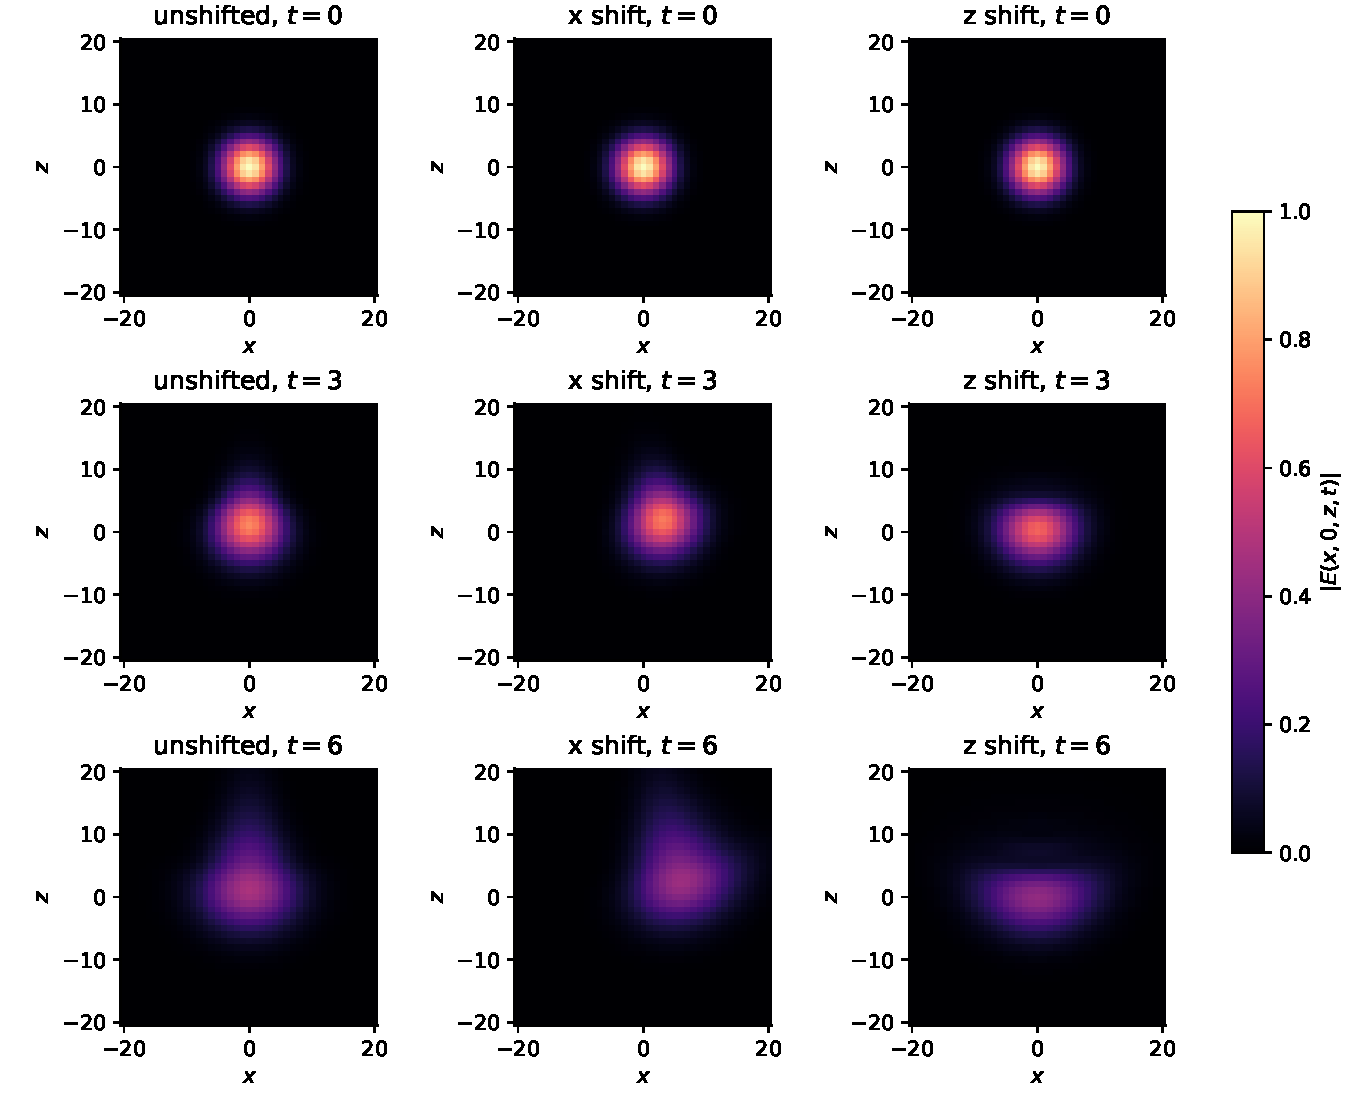
\includegraphics[width=.97\linewidth]{figures/slices.pdf}\end{center}
\textbf{Figure 4.} Magnitude on the $y=0$ plane for $\varepsilon_2=1$. Columns
compare unshifted, $x$-shifted, and $z$-shifted initial spectra. Rows show
$t=0,3,6$. Every panel uses the same color range, making the loss of peak
amplitude visible. The displayed window is $[-20,20]^2$ within the larger
computational box; the color plots are slices of genuine three-coordinate solutions.

Modulation changes propagation as well as deformation. A slice alone can miss
an off-plane maximum, which is why Figure 3 and the table use the full volume.
Full complex fields at $t=6$ are supplied in the accompanying snapshot archive.

\newpage
\section*{4. Directional spreading and generic initial data}
\begin{center}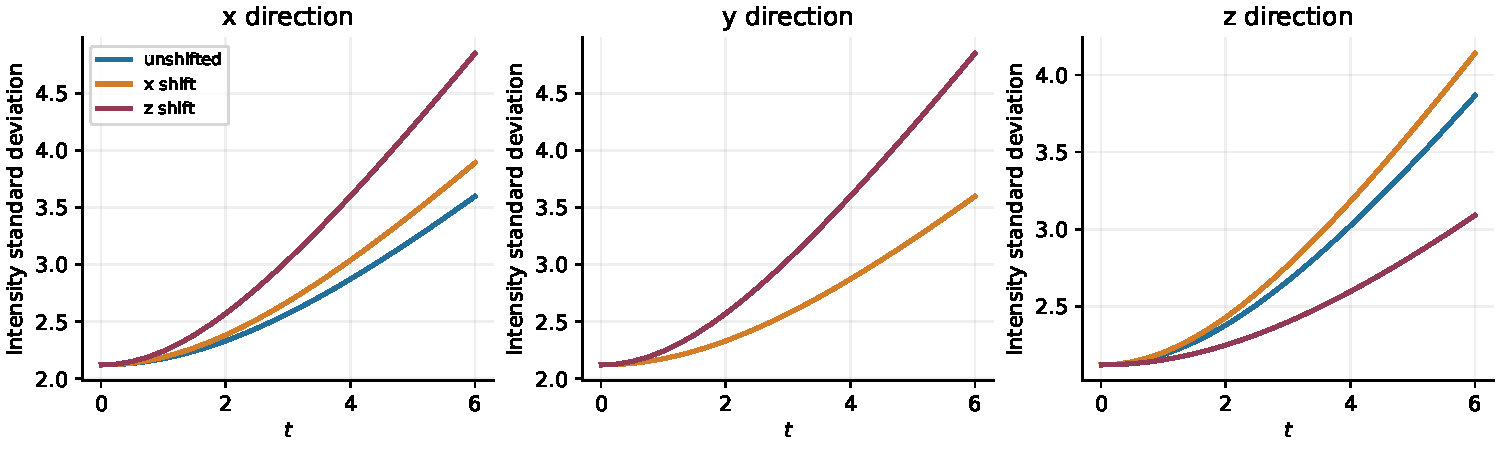
\includegraphics[width=\linewidth]{figures/widths.pdf}\end{center}
\textbf{Figure 5.} Intensity widths for $\varepsilon_2=1$. An $x$-shift breaks
the equality of the transverse widths; a $z$-shift changes both transverse widths
together. Exchanging $x$ and $y$ in the shifted experiment agrees to maximum
absolute field error \SymmetryError.

This behavior is consistent with the group velocity of \eqref{eq:prop}:
\[
 \nabla_{\mathbf k}\omega=
 \bigl(2(1+\varepsilon_1k_z)k_x,\;
       2(1+\varepsilon_1k_z)k_y,\;
       \varepsilon_1(k_x^2+k_y^2)-2k_z+3\varepsilon_2k_z^2\bigr).
\]
Changing $k_z$ changes the transverse dispersion factor itself. Changing $k_x$
also affects longitudinal transport through the $k_x^2$ term. The axes are coupled.

\begin{center}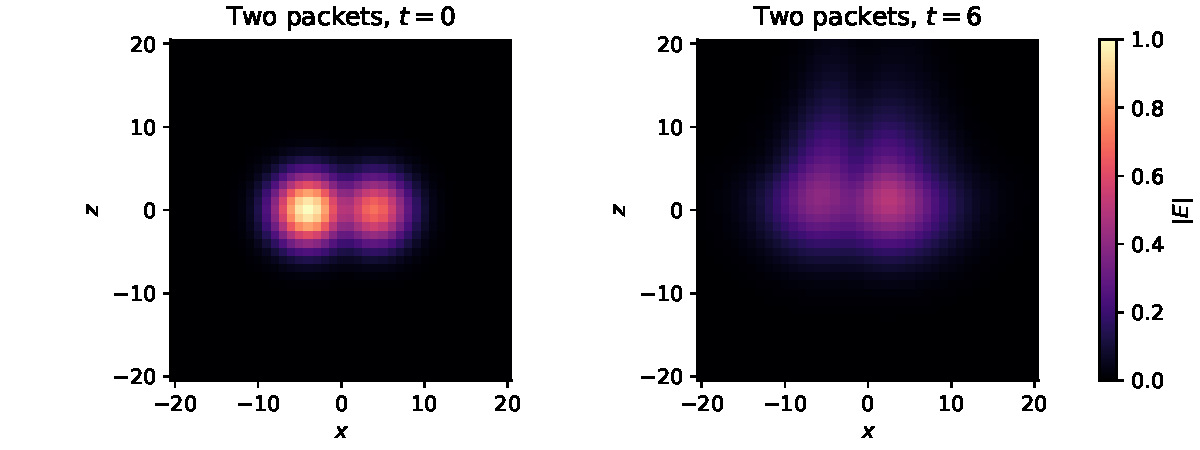
\includegraphics[width=.85\linewidth]{figures/generic.pdf}\end{center}
\textbf{Figure 6.} A non-Gaussian initial profile, propagated with the same solver:
\[
 E_0=e^{-((x+4)^2+y^2+z^2)/18}
       +0.7i\,e^{-((x-4)^2+y^2+z^2)/18},\qquad \varepsilon_2=1.
\]
This example demonstrates that the solver accepts a sampled complex field without
requiring a Gaussian formula. Its separate convergence study is not included here.

\newpage
\setlength{\parskip}{4pt}
\section*{5. Verification and interpretation limits}
\textbf{Algebraic checks.} A periodic plane wave with wavevector $(1,2,-1)$ at
$\varepsilon_1=\varepsilon_2=1$ has $\omega=-2$, hence exact multiplier $e^{2it}$.
The solver agrees at $t=0.73$ to \PlaneError\ in maximum error. Forward/backward
propagation of the $z$-shifted packet gives relative $L^2$ error \ReverseError.
These checks complement conservation, which alone cannot detect a wrong phase sign.

\textbf{Grid refinement.} The table compares the $z$-shifted field at $t=6$ against
a $192^3$ computation on the same length-96 box. The reference is restricted to
the coarse nodes before measuring relative discrete $L^2$ error.
\begin{center}\begin{tabular}{rrrr}\toprule
Grid & $\varepsilon_2=1$ & $\varepsilon_2=-1/3$ & $\varepsilon_2=0$ \\\midrule
\GridRows
\bottomrule\end{tabular}\end{center}
This demonstrates convergence of sampled fields on a fixed periodic box. It does
not imply that a grid maximum equals the continuum supremum. Across all nine final
Gaussian fields, doubling the resolution changes the sampled peak by at most
\PeakPercent\ percent. Figure 3 retains the production-grid maxima.

\textbf{Domain enlargement.} At spacing $0.5$, length-48 and length-72 boxes are
compared to length 96 on the common cube $[-24,24)^3$, using the $z$-shifted field.
A separate check compares each production field to a length-144 box at spacing 1,
restricted to the entire original box. The last column is the worst of all three shifts.
\begin{center}\begin{tabular}{rrrr}\toprule
$\varepsilon_2$ & $L=48$ vs. 96 & $L=72$ vs. 96 & $L=96$ vs. 144 \\\midrule
\DomainRows
\bottomrule\end{tabular}\end{center}
Values are relative discrete $L^2$ differences on the stated comparison regions.
The agreement improves on enlarging the box, but it is evidence on $0\le t\le6$,
not permission to extrapolate indefinitely on a periodic domain.

\textbf{Independent whole-space check.} For the Gaussian, the transverse Fourier
integrals can be evaluated analytically, leaving a one-dimensional adaptive integral
in $k_z$. At $t=6$, we compare the origin, $(3,-2,5)$, and the production peak node
for each of the nine cases. The largest absolute complex-field discrepancy is
\QuadError. Quadrature uses $k_z\in[-5,5]$ with absolute and relative tolerance
$10^{-12}$; Gaussian tails outside this interval are negligible at this precision.
This checks 27 points, not the entire continuum field.

\textbf{Relation to the paper.} Propositions 6.2--6.3 bound a fractional-derivative-weighted
solution in transformed coordinates for $0<\alpha<1$. They do not directly assert
the plotted unweighted peak follows $t^{-(3+\alpha)/3}$. No exponent is fitted here,
and no theorem constant is inferred. Weighted diagnostics and a longer, independently
converged time window are the next experiments.

\textbf{Reproduction.} From the project folder, run the following commands:
\begin{quote}\small\ttfamily
python3 numerical\_solutions.py\\
python3 report/make\_tables.py
\end{quote}
Compile this source from \texttt{report/}. Dependencies are NumPy, SciPy, Matplotlib, and Torch.
The supplied CSV contains all 225 Gaussian norm records; JSON contains checks and
configuration; the NPZ contains nine final Gaussian fields and the two-packet field.
The recorded computation and figure-generation time was \Runtime\ seconds on this
host; this is one CPU run, not a hardware benchmark or a GPU measurement.

\textbf{Source.} R. Mosincat, D. Pilod, and J.-C. Saut,
\emph{On Third Order Nonlinear Schr\"odinger Equations}, supplied manuscript
\texttt{Dysthe3D-2.pdf}, pp. 9--10 and 18--23. No publication status is assumed.
\end{document}
